\documentclass[11pt]{amsart}

% Standard letter size paper with 1inch margins
\usepackage[letterpaper, margin=1in]{geometry}
\usepackage{booktabs} % For better looking tables
\usepackage{xcolor}
\usepackage{pifont}

% Useful packages 
\usepackage{amsmath, amssymb, amsthm, amsaddr}
\usepackage{enumerate, subcaption, graphicx, hyperref}
\usepackage{algorithm}
\usepackage{algpseudocode}
\usepackage{cite}
\usepackage{bm}

\newcommand{\I}{\mathrm{i}}
\DeclareMathOperator{\E}{e}

\title{AMATH 582: Homework 5}
\author{Hunter Lybbert} % first and last name

\address{Applied Mathematics Department, University of Washington, Seattle, WA 
\\ \texttt{hlybbert@uw.edu}}

\date{\today} % you can also just type the date instead of "\today"

\begin{document}

\maketitle

\begin{abstract}
    In this report we compare and analyze the merits of Convolutional Neural Networks (CNNs) against our previous work with the Fully Connected Network (FCN).
    An FCN with the best hyperparameter configuration from report 4 is trained with multiple different total number of weights.
    Additionally, hyper-parameter tuning is conducted for the CNN.
    Finally different CNNs are trained with different total numbers of weights but with the best hyperparameter configuration from the previous step.
    An analysis of the costs and benefits of these two models is presented, primarily focused on the number of weights, training time, and model accuracy on the test set.
\end{abstract}

\section{Introduction and Overview}\label{sec:Introduction}
Continuing our study of deep learning, the field of neural network based model architecture, we turn our attention to Convolutional Neural Networks (CNNs).
But first, let's review our basic setup.

Again, we are concerned with a supervised learning problem, given a collection of $N$ data points with labels in classification or target values in a regression setting $$\big\{(\bm{x_0}, y_0), (\bm{x_1}, y_1), ..., (\bm{x_{N-1}}, y_{N-1})\big\}.$$
The data is denoted as a matrix $X$ and a vector of target values or class labels $\bm y$.
We then are looking for a function $f$ which takes in the training data and most accurately predicts the target values or class labels, written in optimization form we are looking for the following
\begin{equation}
f_{MLE} = \underset{f}{\rm argmin } \frac 1 {2 \sigma^2}|| f(X) - \bm y ||_2^2
\label{eq:basic_ml_setup}
\end{equation}
where $\sigma^2$ is the variance of the normally distributed error terms $\epsilon \sim \mathcal N (0, \sigma^2)$ defined by $\epsilon_i = y_i - f(x_i)$
So said another way we are trying to minimize our errors in the classification task.
The specific class of functions $f$ to be considered to solve the problem is a neural network, specifically we evaluate and compare FCNs to CNNs.
We will treat the theoretical background of these methods in the next section \ref{sec:theory}.

Before proceeding, we would like to acknowledge the critical use of the following packages in our analysis.
Namely, NumPy for many computational tools \cite{harris2020array} and Matplotlib was used to create all plots and animations \cite{Hunter:2007}.
Addiitonally, PyTorch \cite{Ansel_PyTorch_2_Faster_2024} was crucial for easily implementing the desired architecture while Ray Tune \cite{liaw2018tune} was used to help with hyper parameter tuning.

\section{Theoretical Background}\label{sec:theory}
For a general theoretical background on neural networks and basic hyperparameters please refer to the report from homework 4.
We presented our theoretical background clearly there.
Instead of repeating the information about gradient descent, back propogation, optimizers, learning rates, and dropout etc. in this report again, we will focus on the unique architectural considerations of a convolutional neural network.

Traditionally in mathematics a convolution is denoted by the two functions $f * g$ which usually means:
$$(f*g)(t) = \int_{-\infty}^\infty f(\tau) g(t - \tau) d \tau.$$
Another form of convolution that many are familiar with (perhaps just not by that name) is multiplying out two polynomials (where each term in one polynomial is multiplied by each term in the other polynomial)
\begin{align*}
& (a_0 + a_1x + a_2x^2) (b_0 + b_1x b_2x^2 + b_3x^3 + ...) \\
&= a_0b_0 + (a_1b_0 + a_0b_1)x + (a_2b_0 + a_1b_1 + a_0b_2)x^2 + (a_3b_0 + a_2b_1 + a_1b_2)x^3 + ...
\end{align*}
For more details about the connection between the polynomial multiplication type of convolution and our convolution of interest in CNNs see this lovely video \cite{youtube_video}
The convolution we care about in particular is a method of sliding a filter of a specified dimension across our matrix or tensor of data and multiplying the values of the filter with the values of our data and producing new outputs based on this calculation.

In particular, our fully connected neural network created a weighted sum by multiplying each node from the previous layer by a weight and summing it up to pass that value along to the next layer.
This convolution allows us to pass in images or other data which has some spatial orientation and applying these weights to just a small subset of the previous layers data at a time to generate the next layer of data.
CNNs perform exceptionally well on image data because they preserve and can account for this spatial relationship between data in different pixels.

\begin{figure}[h]
	\centering
	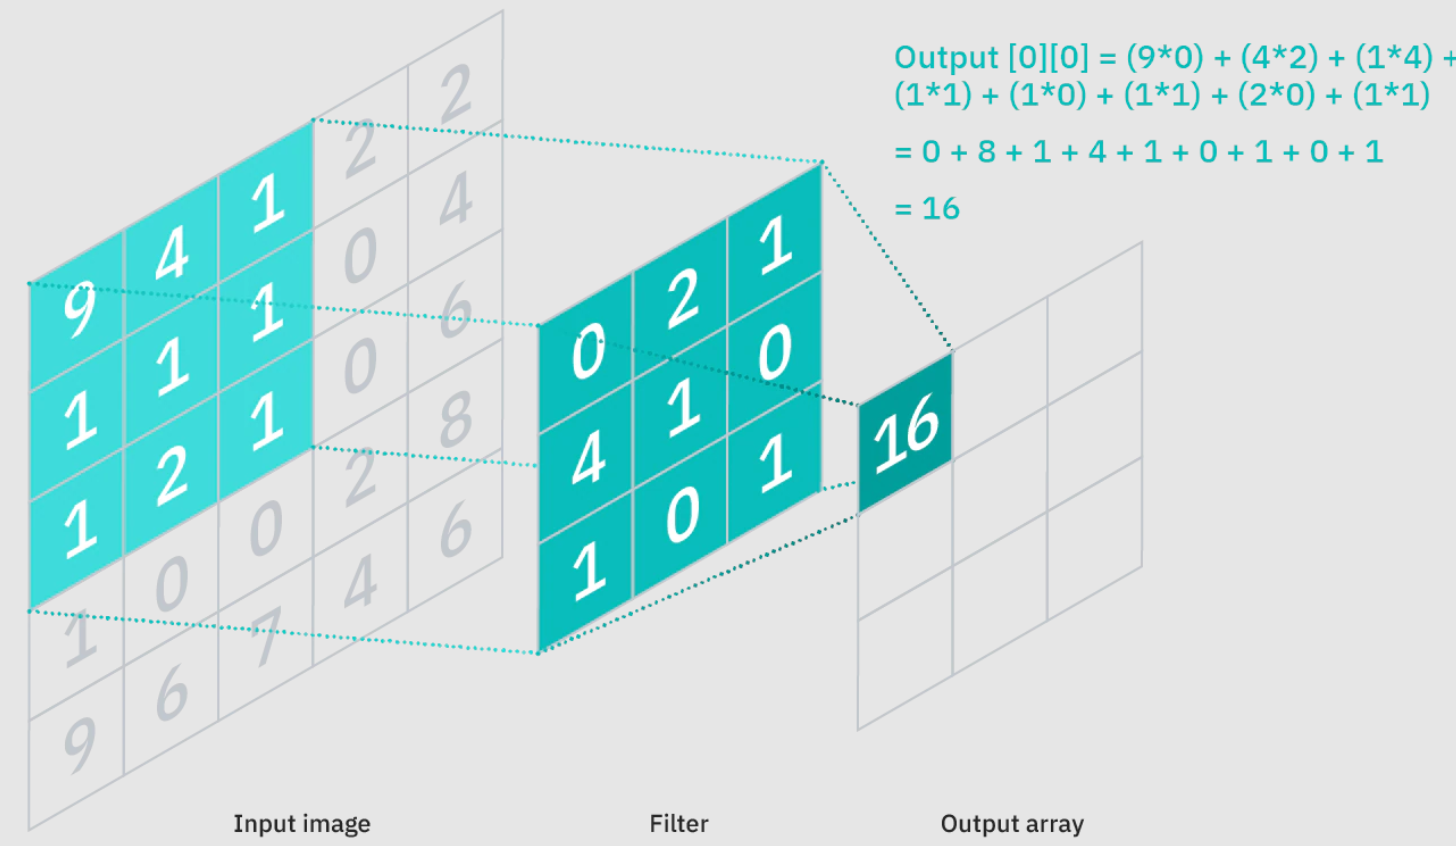
\includegraphics[width=.6\textwidth]{../visualizations/convolution_visualization.png}
\caption{This is a visualization of how a filter is applied to a previous layer to produce the next layer in a CNN, it is borrowed from this resource \cite{vitalfluxRealWorldApplications}.}
    \label{fig:conv_viz}
\end{figure}

In Figure \ref{fig:conv_viz}, we demonstrate how the 3x3 filter is applied to the upper left hand corner of the input layer.
This convolutional filter is the basic component of a CNN.
It introduces a new set of architectural parameters and considerations including
\begin{itemize}
\item The number of convolutional layers (depth of the network)
\item The dimension of each convolutional filter (usually odd 3, 5 or 7)
\item The number of output channels (aka the number of filters applied to each input channel) at each layer
\item Stride length
\item Padding
\end{itemize}
We haven't discussed stride or padding yet, but we will describe their role presently.

As demonstrated in Figure \ref{fig:conv_viz}, applying the filter to the top left part of our input produces the top left pixel or value of the output channel.
Now the next set of values we apply the filter to depends on the parameter stride.
Stride is the length of the steps taken in both the sidewise and vertical directions.
A stride of one would move the filter over just one column to produce the next output value, while a stride of two would move the filter over two columns to produce the next output value.
Next, padding is a method to help avoid having the image or data continue to shrink after each convolutional filter is applied.
Once again, as seen in Figure \ref{fig:conv_viz}, our setup as is reduced the data from 5x5 to 3x3.
Using a padding value of 1 would add a buffer of 0's around the edge of our data.
The input data would artificially be 7x7 and applying our 3x3 filter with a stride of one would give us an output image or data of shape 5x5 effectively preserving the original image or data dimension through the convolution.
The dimension of the output layer after applying a given filter with it's set of parameters is given by:
$$
n^{[\ell]} = (n^{[\ell - 1]} +2p - f)/s +1
$$
where the dimension of the data in layer $\ell$ is ($n^{[\ell]}$, $n^{[\ell]}$), the padding value used is $p$, the dimension of the filter is $f$, and the value of stride is $s$.
Note in our examples, we have mentioned before we have an input layer of 5x5, without padding ($p = 0$) applying a 3x3 filter to the layer with a stride of 1 would give us
\begin{align*}
n^{[\ell]} &= (n^{[\ell - 1]} +2p - f)/s +1 \\
n^{[\ell]} &= (5 +2(0) - 3)/1 +1 \\
n^{[\ell]} &= (5 - 3)/1 +1 = 3.
\end{align*}
However, with padding of one we would end up with $n^{[\ell]} = (5 +2(1) - 3)/1 +1 = (7 - 3)/1 + 1 = 5$, effectively preserving the dimension of the input through to the output.
The values of the entries of the various convolutional filters are the weights which are getting updated throughout the training process using Gradient Descent and back propagation.

Additionally, there are some static layers which are not updated with back propagation such as pooling layers.
A pooling layer, similar to a convolutional layer is a filter of some sort being passed over the data reducing its dimension or compressing the data in some manner.
A couple of common ones to mention are average pooling and max pooling.
These are commonly 2x2 filters which produce a single value output based on the type of pooling.
Max pooling would pass along the max value from the 2x2 pixels it is passing over, while average pooling would pass along the average of the 4 values being considered at that moment.


Finally, as mentioned in the list of considerations for CNNs, we also can decide how to increase the number of channels in each layers.
A regular RGB image has three input channels, so a 3 dimensional filter will be applied to the collection of data with the extra dimension corresponding to the input channel dimension.
If the desire is to have the output channels to be the same size then there will only be one of these filters.
However, commonly we want to increase the number of channels to capture more complex information as the data moves through the CNN.

\section{Algorithm Implementation and Development}\label{sec:algorithms}
In order to train a CNN we began by creating a model class using PyTorch's \cite{Ansel_PyTorch_2_Faster_2024} many built in methods and classes.
This time we manually experimented with different number of convolutional layers until we settled in on our basic architecture (3 convolutional layers and a fully connected layer).

I did not try to use Ray Tune \cite{liaw2018tune} again, but rather I generalized the model training python class I created in homework 4 to be able to apply it to both the CNN and FCN.
This generalizing of the python class led me to relearning a bit about python class inheritance and was a good exercise in trying to generalize my code.
This generalized class still managed the experiments for me and recorded results, total number of weights, training time, and other parameter settings to a \textit{json} file.
This allowed me to train many models over night and analyze the results the next day and refer back to them in the future as well.
It is all easy to use and very reproducible.

After some manual experimentation with different model architectures I found the following

Due to the large number of hyper parameters it is an overwhelming amount of information to specify in each plot for each loss or accuracy curve.
Therefore, I have labeled plots with experiment numbers and mean accuracy across test set.
For select models I will detail their exact configuration in the next section \ref{sec:results}, while others can be looked up in the repo directly on \href{https://github.com/hunter-lybbert/uw-central/blob/main/data_analysis/hw_05/experiments/experiments.json}{GitHub}.

\section{Computational Results}\label{sec:results}
Our carefully crafted tables and figures can largely speak for themselves, but I will highlight several key results and findings from the actual training process.
The first big result from training the CNN was that the model quickly overfit with just convolutional and pooling layers.
This was clear because in the training accuracy achieved 100\% for the last several epochs.
Additionally, for the models that hit this, their test accuracy was lower like 88\% or so which we knew the CNN could do better than that.
However, after implementing batch normalization between convolutional layers and adding dropout to the single fully connected layer at the end of the model, we were able to mitigate the overfitting as best we could, soon achieving model accuracies closer to 92\%.
For further analysis of the results, hyperparameter tuning, and comparisons, please peruse the remaining figures and tables.

\begin{table}[h]
    \centering
    \begin{tabular}{|l|c|c|c|c|c|c|c|c|c|c|} % 'l' for left-aligned, 'c' for center-aligned columns
        \hline
        \textbf{Ep.}
        & \textbf{Arch} & \textbf{W. Init}
        & \textbf{B. Norm} & \textbf{Drop}
        & \textbf{Optim} & \textbf{lr}
	& \textbf{$\bm \mu$ (Test Acc)}
        & \textbf{$\bm \sigma$ (Test Acc)} \\ 
        \hline
        50 & [1024, 256]  & Kaiming & True & [0.5, 0.5] & Adam & 0.001 & 0.9030 \textcolor{red}{\ding{72}} & 0.0021 \\
        \hline
    \end{tabular}
    \caption{This was the configuration that was best from the last report in hw 04.
    Therefore it was the base setup for the FCN's trained in this hw 05, however, with the necessary adjustments due to weight count constraints.}
    \label{tab:best_model}
\end{table}

\begin{table}[h]
    \centering
    \begin{tabular}{|l|c|c|c|c|c|c|c|c|c|c|} % 'l' for left-aligned, 'c' for center-aligned columns
        \hline
        \textbf{ID} & \textbf{Model} & \textbf{Weights}
        & \textbf{Time} & \textbf{Ep.}
        & \textbf{Optim}
        & \textbf{lr} & \textbf{W. Init}  & \textbf{$\bm \mu$ (Test Acc)}
        & \textbf{$\bm \sigma$ (Test Acc)} \\
        \hline
        49 & CNN (100k) & 108,814 & 0:06:15 & 50 & Adam & 0.001 & Xavier & 0.9236 \textcolor{red}{\ding{72}} & 0.0167 \\
        \hline
        56 & CNN (10k) &   9,980 & 0:04:02 & 50 & Adam & 0.001 & Xavier & 0.9002 & 0.0229 \\
        \hline
        57 & CNN (20k) & 20,071 & 0:04:15 & 50 & Adam & 0.001 & Xavier & 0.9091 & 0.0151 \\
        \hline
        58 & CNN (50k) & 50,392 & 0:05:19 & 50 & Adam & 0.001 & Xavier & 0.9152 & 0.0188 \\
        \hline
        59 & FCN (50k) & 52,842 & 0:02:30 & 50 & Adam & 0.001 & Kaiming & 0.8802 & 0.0158 \\
        \hline
        60 & FCN (100k) & 109,770 & 0:02:32	 & 50 & Adam & 0.001 & Kaiming & 0.8889 & 0.0211 \\
        \hline
        61 & FCN (200k) & 202,974 & 0:02:32 & 50 & Adam & 0.001 & Kaiming & 0.8965 & 0.0188 \\
        \hline
    \end{tabular}
    \caption{
    After performing Hyperparameter tuning to determine the best settings for out CNNs, we trained models with 100k, 50k, 20k, and 10k weights.
    Using the configuration from Table \ref{tab:best_model} (best from homework 4) we trained 3 FCN's each with 200k, 100k, and 50k weights in each model.
    Notice that training time increases very rapidly for the CNN as the number of parameters increases, while the FCN training time is almost constant (at least at the scale and for the experiments we conducted.
    Finally, notice how even the smallest CNN outperforms the FCN on the test set accuracy, let alone how high the test accuracy is with the 100k weights CNN.}
    \label{tab:diff_weights}
\end{table}

\begin{figure}[h]
    \centering
    \begin{subfigure}{0.49\textwidth}
        \centering
        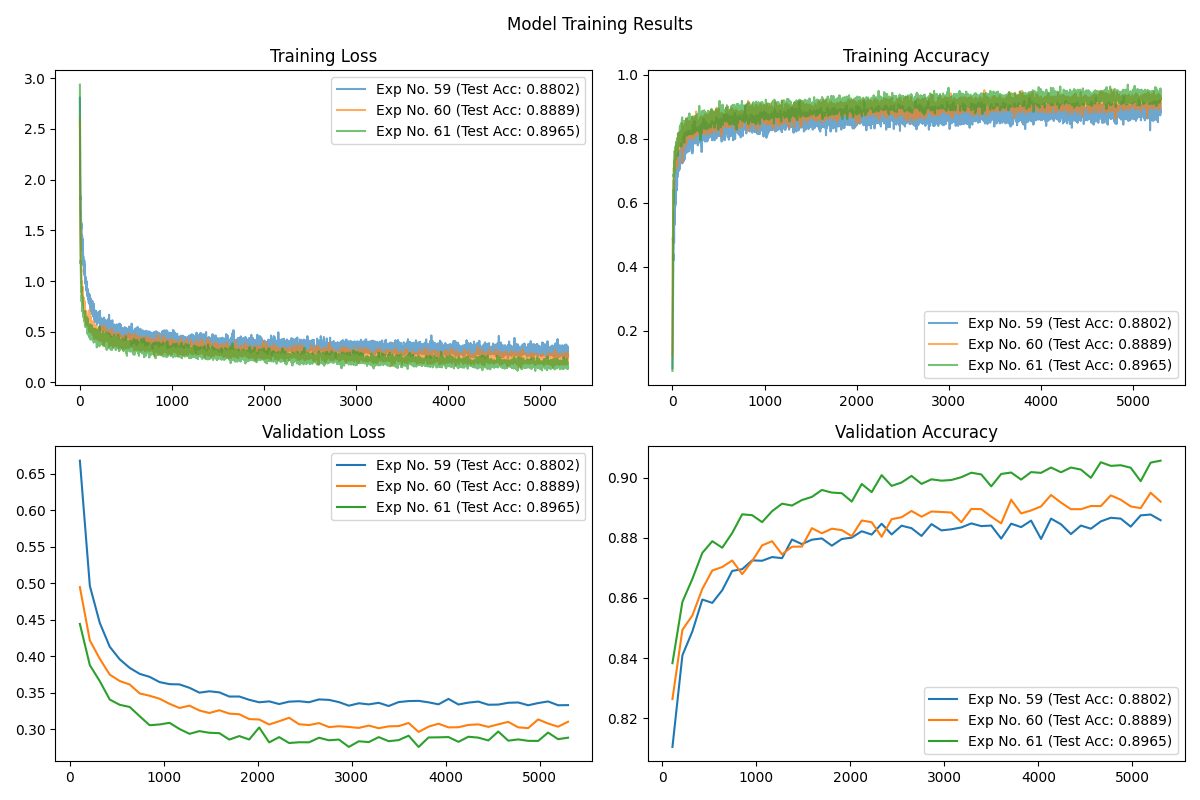
\includegraphics[width=.9\textwidth]{../visualizations/model_training_results_vis_2.png}
        \label{fig:image1}
    \end{subfigure}
    %\hspace{1mm}
    \begin{subfigure}{0.49\textwidth}
        \centering
        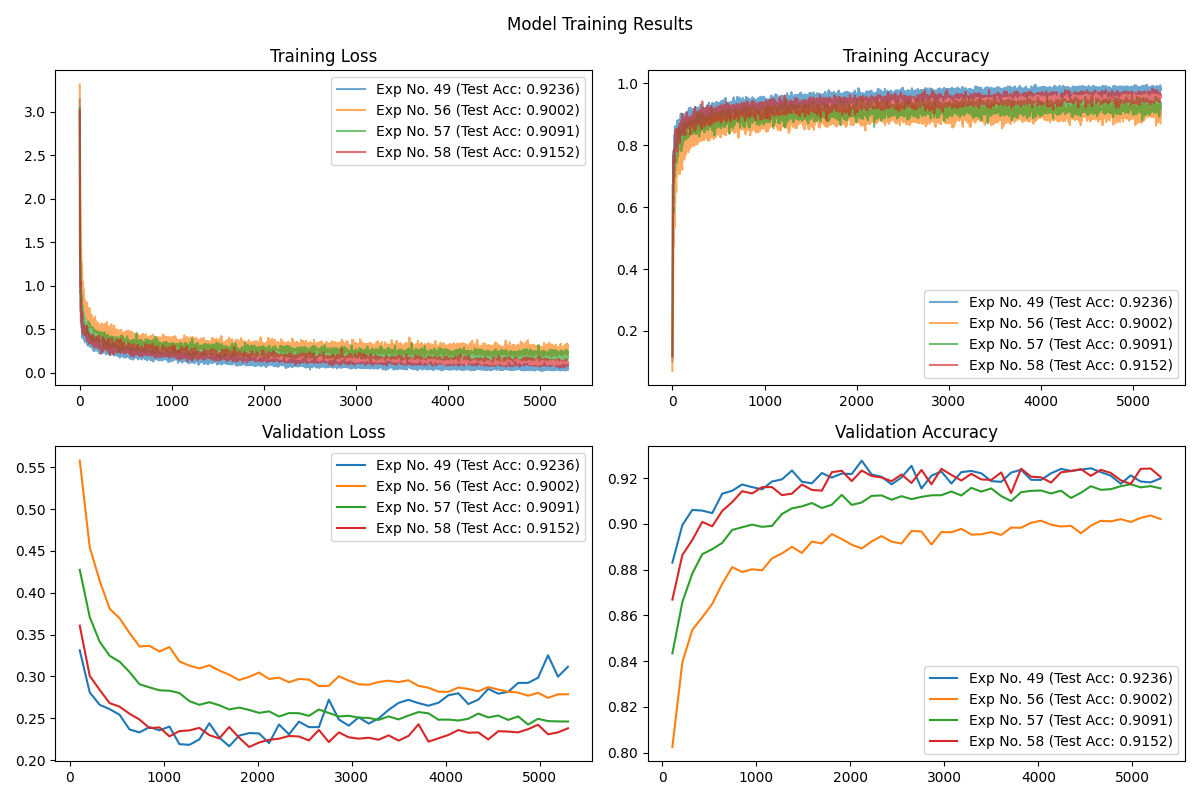
\includegraphics[width=.9\textwidth]{../visualizations/model_training_results_vis_3.png}
        \label{fig:image2}
    \end{subfigure}
    \caption{On the left we have the 3 different FCNs which are all the same except different total number of weights, compare to Table \ref{tab:diff_weights}.
    On the right are the 4 different CNNs trained with the same parameter settings except they vary the total number of weights, compare to Table \ref{tab:diff_weights}.}
    \label{fig:f0}
\end{figure}

\begin{figure}[h]
	\centering
	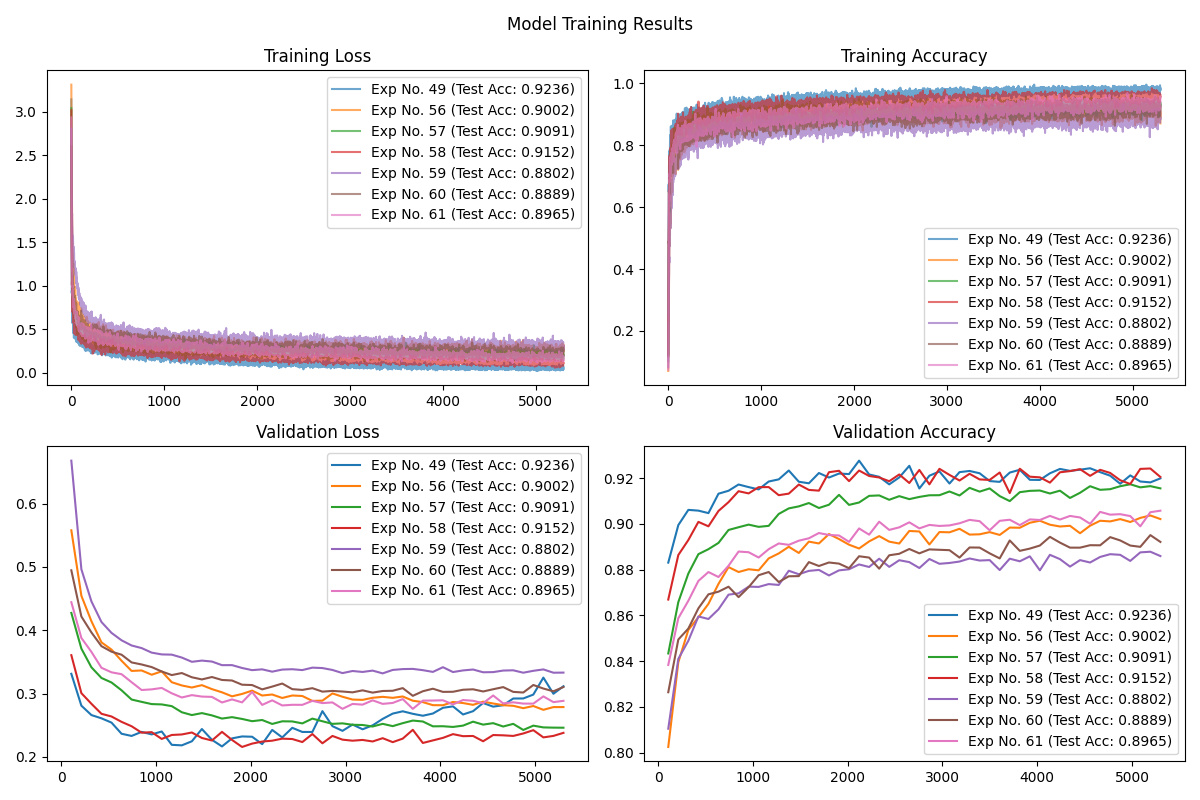
\includegraphics[width=.6\textwidth]{../visualizations/model_training_results_vis_1.png}
\caption{This is a visualization of all of all models in Table \ref{tab:diff_weights}.
	They were visualized separately in Figure \ref{fig:f0}.}
    \label{fig:f1}
\end{figure}

The last piece to discuss in our computational results is the visualization of the feature maps in our model.
In Figure \ref{fig:feat_maps}, we can see the feature maps for each of the 3 convolutional layers in one of our CNNs we trained.
Not only are these fun and interesting to look at, but it conveys some assurance that indeed the model is cluing into some key features or parts of the input image to help it make an accurate prediction.
While some channels appear to be cluing into the edges of the sweatshirt image others are focused on the contrast between the backdrop and the item.
I can see how in a more complex problem with more diversity in the input images, we might see a wider variety of shapes and features highlighted in the feature maps.
Overall, this was a really cool part of the project and we are proud to share it in our report.

\begin{figure}[h]
	\centering
	\begin{subfigure}{0.49\textwidth}
    		\begin{subfigure}{\textwidth}
        			\centering
			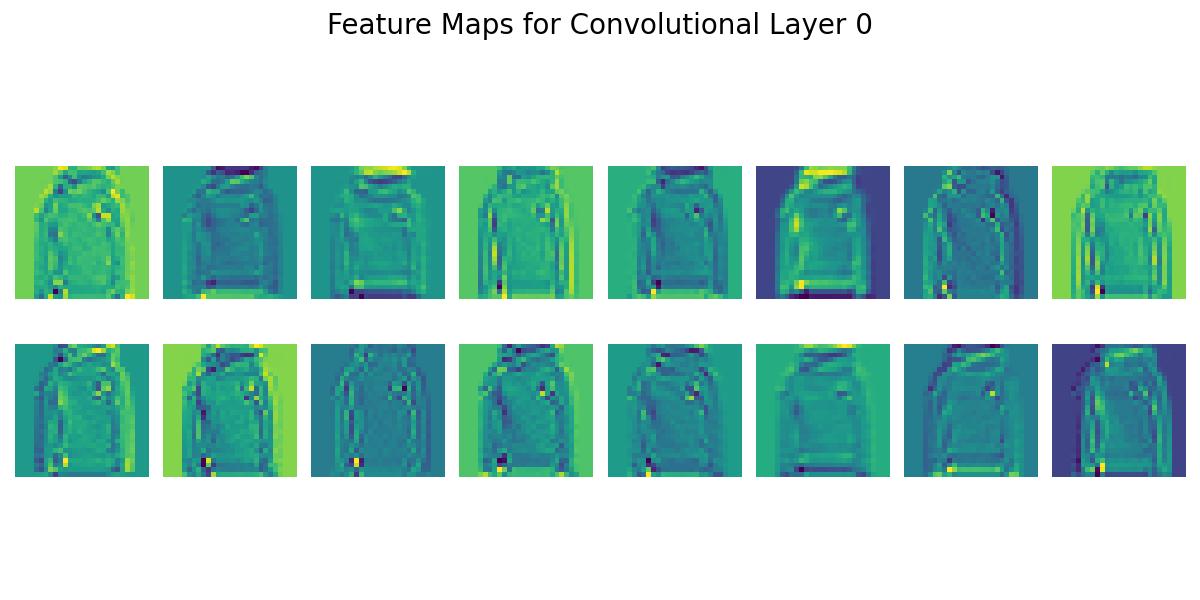
\includegraphics[width=.9\textwidth]{../visualizations/feature_maps_conv_layer_0.png}
	    	\end{subfigure}
		\begin{subfigure}{\textwidth}
			\centering
			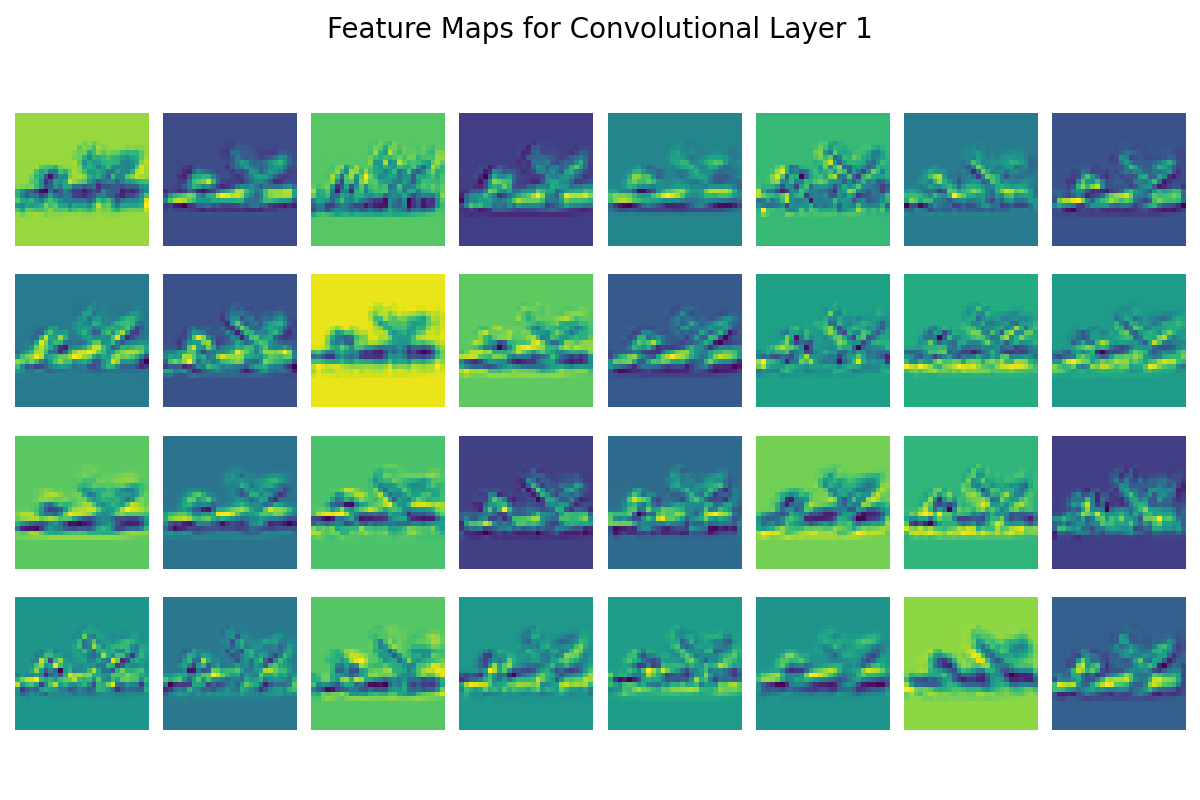
\includegraphics[width=.9\textwidth]{../visualizations/feature_maps_conv_layer_1.png}
		\end{subfigure}
	\end{subfigure}
	\begin{subfigure}{0.49\textwidth}
		\centering
        		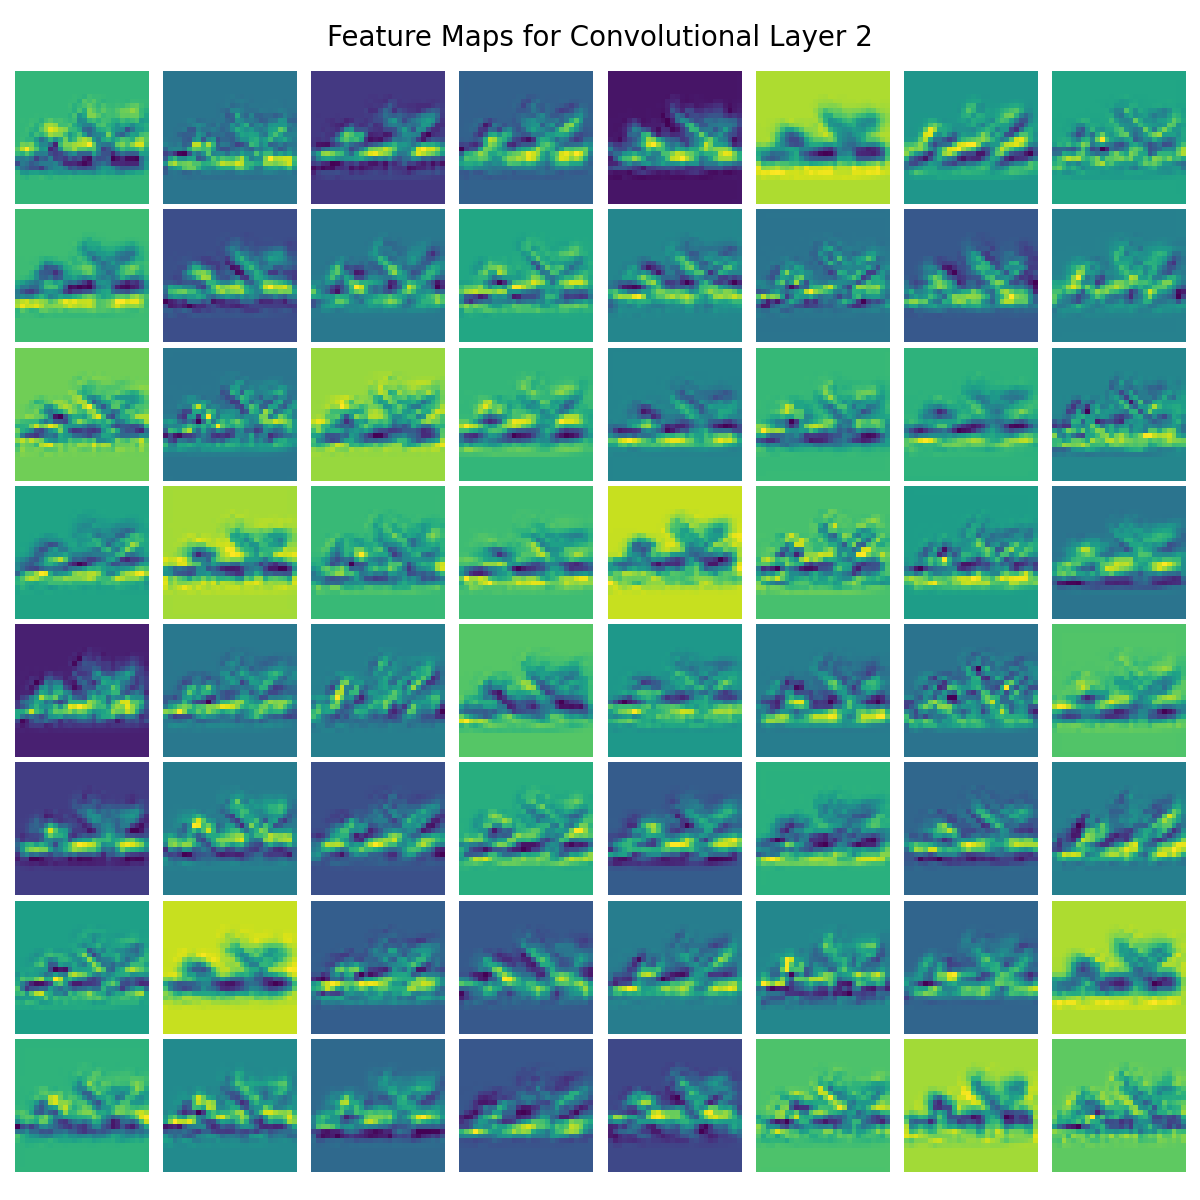
\includegraphics[width=.9\textwidth]{../visualizations/feature_maps_conv_layer_2.png}
	\end{subfigure}
\caption{Feature maps from each of the 3 layers of our model.}
\label{fig:feat_maps}
\end{figure}


\section{Summary and Conclusions}\label{sec:conclusions} 
From our analysis we determined that in terms of accuracy on the test set the CNN is the preferred model architecture. However, the CNNs training time dramatically increased compared to the fully connected networks.
Despite this draw back, the CNN is still likely the preferred model for this problem especially considering the models performance even when only using 10k weights.
When using 5\% of the weights of the biggest FCN (200k) we tested, the 10k CNN still outperformed it on the test set.
These accuracy gains with respect to minimal number of parameters required is why we would choose a CNN.
However, if we needed to perform a task with a larger dataset, larger model architecture, etc. the temporal complexity of the CNN would start to be a bigger consideration.
Again, if one is curious to look through more of the results mentioned in the report and those not included here, it is recorded here on \href{https://github.com/hunter-lybbert/uw-central/blob/main/data_analysis/hw_05/experiments/experiments.json}{GitHub}
This was an excellent introductory experience into building, training, and evaluating a CNN versus traditional FCN.

\section*{Acknowledgements}
The author is thankful to Jaxon Tuggle for offering regular feedback and counsel when interpreting results and clarifying the implications and merits throughout the hyperparameter tuning process.
We would also like to thank Professor Eli Shlizerman for carefully instructing us in class.

\bibliographystyle{abbrv}
\bibliography{references_hw5} % make sure this matches the .bib file for your corresponding document. You also have to maintain your references in the .bib file 

\end{document}
